\chapter{Referencial Teórico}
Este capítulo apresenta os principais conceitos explorados para o desenvolvimento do presente trabalho, desde conhecimento das tecnologias necessárias quanto conceito imprescindíveis para a construção da proposta até o estudo para o desenvolvimento do projeto. Com o intuito de fundamentar a
metodologia, foram estudados os conceitos e características do visagismo, grupos de pele, características e grupos cromáticos de pele, escalas de tons. Após são apresentados os conceitos e técnicas de processamento digital de imagens relacionadas ao sistema de cores, técnicas de classificação automática e tratamento digital de imagens.

A percepção visual da cor da pele desempenha impacto no papel social de um indivíduo perante a avaliação de etnia, idade, saúde e atratividade. A cor da pele do indivíduo pode ser interpretada como indicador de sua história, decorrente da sua inserção em determinado grupo social. Sendo assim,  ela não só configura o fator genético, mas como o fator sociocultural que pode influenciar no modo que o indivíduo consome. Assim como, altera a percepção e as preferências de produtos entre os usuários de maquiagem, especialmente na escolha de maquiagens como o tom de base a ser utilizado. 

Nos países asiáticos, como o Japão, o padrão de beleza é a pele clara, onde é comum a venda de produtos que clareiam e protegem a pele contra raios UV, pois a pele branca é tratada como nobre. Já em países ocidentais tem se tornado comum a discussão de representatividade, principalmente da pele preta. No Brasil e Estudos Unidos, as marcas veem abordando o mercado com novos produtos que possuem faixas de cores mais abrangentes. Como a empresa Fenty Beauty que se destacou no mercado por ter seu primeiro lançamento de 50 tons de base e a empresa Bruna Tavares, no Brasil, que seu primeiro lançamento continha 30 tons, algo revolucionário para o mercado. Porém, além do problema das cartelas de cores, há a falta de padronização na nomenclatura para as cores, dificultando para o consumidor encontrar uma mesma cor em diferentes marcas.

A base pode ser líquida, em pó ou creme e é o primeiro passo para na maquiagem facial.  E são utilizadas para deixar a pele uniformizada, cobrindo manchas, alterando o tom e a textura para a impressão de uma pele mais saudável e jovem \cite{Foundation}. O tom de base é parte fundamental de uma maquiagem que pode ou não criar um efeito máscara no cliente devido à discrepância de coloração de pele que pode gerar entre o corpo e face.

A escolha do tom de um produto, como a base, pode ser alterada conforme o tom e subtom que a pessoa possui. Isso se deve a tonalidade do produto impactar a percepção e compatibilidade de acabamento entre a pele e o produto, que se não semelhante ou igual transmite efeitos indesejados como estranheza pela distinção entre áreas de rosto, colo e pescoço. Por isso, a escolha de não só um tom semelhante à pele, mas o subtom do produto, sendo ele quente, frio ou neutro, impacta a imagem a ser transmitida e elas devem ser avaliadas separadamente. De acordo com \cite{Maquiagem_técnicas_referências_e_atuação_profissional}  o  subtom  não tem relação com o tom de pele nem a etnia, mas as substâncias como a melanina. A melanina é dividida em duas substâncias, sendo elas a fenomelanina que dá pigmentação amarelada e vermelhada a pele e a eumelanina que acentua tons marrons e pretos.

\section{Visagismo}
O visagismo foi criado por Fernand Aubry em 1937 e tem origem do termo \textit{visagisme}, palavra que, em francês, significa rosto. Contudo, Fernand Aubry não publicou livros, ou definiu o conceito do visagismo. Contudo, entendeu-se a partir de fragmentos de suas aulas de maquiagem que ele acreditava que o profissional de beleza deveria criar em seus clientes uma imagem harmônica e equilibrada visualmente e que essa imagem deveria expressar uma personalidade \cite{Visagismo_Harmonia_e_Estetica}.

O visagismo foi introduzido no Brasil a partir do livro de Philip Hallawell, que define como a técnica que compõe a imagem pessoal, revelando as qualidades de uma pessoa conforme as suas características físicas e princípios da linguagem visual que se deseja expressar. Essa técnica promove a arte visual, propondo uma relação entre emoções e personalidade, com foco na construção da imagem e beleza \cite{Visagismo_Harmonia_e_Estetica}. Assim, a técnica permite que os profissionais da beleza utilizem do seu conhecimento técnico para auxiliar o seu cliente a definir e se expressar através da sua imagem. Além disso, o conceito do visagismo surge para acabar com a padronização do conceito de beleza\cite{Visagismo}. 

\subsection{Caracterização cromática de pele}
O rosto é o local onde as pessoas se identificam, e qualquer alteração na sua aparência pode alterar essa identificação. Por isso, a relevância do visagismo, pois mudanças na aparência podem influenciar negativamente na vida profissional ou pessoal do indivíduo, assim como o uso ou não de maquiagens \cite{Respostas_Emocionais_Implícitas_Julgamento_da_Atratividade_Facial_em_Faces}. No caso da análise da cor da pele, a coloração pessoal, no visagismo, busca-se identificar as cores que harmonizam com a pele e a realçam com o subtom de pele de cada
pessoa \cite{A_influencia_da_coloração_pessoal_na_autoestima_e_autoimagem}. Para isso, são analisadas as cores superficiais e a temperatura da pele. A cor superficial nas peles brancas se referem ao tom amarelado ou avermelhado; e nas peles negras, amarelado, avermelhado ou marrom-escuro. Para a temperatura da pele há as cores quentes como o laranja, amarelo e vermelho-alaranjado ou vermelho cádmio e frias, como o magenta, roxo, verde e azul. \cite{Visagismo}. Além disso, há a possibilidade harmonizar a pele fria com a cor prateada e peles quentes com a cor dourada.Assim como pode ser analisado, as veias do antebraço apresentarem tonalidades verde ou amarelada, sendo a pele  quente e se manifestarem o azul ou rosada o tom é frio. 

Segundo \cite{Visagismo} para definirmos a cor de pele deve-se ser identificado o tom de pele, sendo ela clara ou escura. Algumas peles negras podem ser confundidas com peles brancas, mas possuem características bem distintas. Em seguida, a temperatura da pele, nesta análise, deve se aproximar da pele uma amostra de cor bege e outra branca, onde peles quentes combinam com a cor bege, enquanto as peles frias combinam com branco e peles neutras combinam com ambas as cores.E finalmente, a estação da pele, no qual a classificação de cada tonalidade de pele é baseada em estações e dividida entre peles brancas e negras.

\subsection{Grupos cromáticos}
Para a coloração pessoal no visagismo há a classificação das cores da pele com referências as estações do ano, pois todas as peles se identificavam com as cores da natureza e nela estão presentes as cores frias e quentes. De acordo com \cite{Visagismo_Harmonia_e_Estetica}, há quatro classificações para tons de pele, sendo elas primavera, outono, inverno e verão. Na classificação de peles quentes temos consoante as estações do ano há a primavera e outono, e para peles frias as estações de verão e inverno. Na análise de coloração pessoal também são consideradas a coloração de cabelo e de olhos e seu realce quando comparados com outras tonalidades, sendo elas proveniente de roupas, acessórios ou mesmo da maquiagem utilizada.

Para as categorias quentes a classificação da primavera as tonalidades de pele, o tom de pele básico é o dourado amarelado e quando se expõe ao sol, produz um bronzeado dourado. Para a pele outono há a classificação dos avermelhados. As pessoas mais claras que possuem esse tipo de pele, quando se expõem ao sol, se queimam facilmente, mas é raro que consigam se bronzear. As pessoas com a tonalidade mais escura ficam com um bronzeado acobreado. Existem dois tipos da pele outono: a pele mais clara e mais escura. 

Para as categorias frias a classificação do tipo inverno são frias e de categoria amareladas, podendo ter o fundo roxo. São opacas, pálidas e, quando se expõem ao sol, ficam com o tipo de bronzeado café, porém, podem escurecer, ficar manchadas e não absorver a cor. As peles do tipo verão são frias, mais delicadas e tendem a ser rosadas com o fundo azulado. Quando se expõem ao sol, queimam com facilidade, porém, não se bronzeiam, têm o bronzeado neutro. 

As peles negras também são muito variadas, vão desde as mais claras, sendo acinzentadas, amareladas, às escuras, sendo avermelhadas, e as muito escuras, sendo azuladas. Podem ser classificadas em tipos frios e quentes. Peles negras contêm muitas cores na sua composição, além da cor de base por serem mais escuras, as peles negras não miscigenadas têm pouco, ou nada, de branco. Todas as peles negras derivam do marrom, variando entre tons de dourado até os tons azulados. Em pessoas com a tonalidade de pele mais clara, ou seja, pessoas mais miscigenadas, existe mais branco, o que pode resultar em um tom neutro ou mais acinzentado. Para a pele negra são classificadas em tonalidades Nilo, Jazz, Saara, Calipso e Spike.

O tipo Nilo se refere a tonalidade neutra da pele e tende a ser uma coloração fria, mais claro e aproximando-se da cor de marfim. O fundo é azul-claro cinzento, porém não tem semelhanças com a pele verão. As peles negras da tonalidade Blues têm o fundo azul, muito escuras e frias. O tipo de pele jazz é escuro, da cor de chocolate ou café, porém mais claro que o tipo blues. Seu fundo é o verde, o que o torna frio. Já o tom Saara tem como característica a cor amarelada clara neutra. Pode parecer com algumas peles do tipo inverno, já que tem o fundo roxo. A pele do tipo calipso tem tonalidade dourada, quente e com fundo terra de siena natural, que se assemelha à pele primavera mais escura. Essa cor de pele é luminosa, vibrante e de tom médio. Tem características de cores quentes e parece estar bronzeada todo o tempo. E, a pele do tipo Spike, têm fundo verde terra, são uma pele avermelhada e se assemelham ao tipo de peles mais escuras, como o tipo outono \cite{Visagismo}. 


\section{Escalas de Tom de Pele}
 
A cor de pele está relacionada a pigmentação herdada geneticamente e da cor induzida pela exposição solar. Para seu estudo há diversas classificações e escalas de tom de pele que se referem a tonalidades agrupadas de acordo com certas características como por sensibilidade a luz ultravioleta, por região geográfica e etnia. A seguir, serão abordados as principais escalas presentes no trabalho.


\subsection{Escala de Fitzpatrick}
A escala de Fitzpatrick é uma ferramenta dermatológica reconhecida internacional para classificação do tipo de pele e sua sensibilidade à radiação ultravioleta. Esta escala de classificação originou-se em 1975 desenvolvida pelo médico dermatologista Thomas B. Fitzpatrick e  utiliza seis classes de cores de pele para descrever o comportamento da pele pelo bronzeamento. Conforme a Figura \ref{fig:x fototipo_fitzpatrick},  por exemplo,  o  Tipo  I  é  para  a  pele  muito  clara, que sofre queimaduras e não se  bronzeia, enquanto   o   Tipo   VI,   corresponde   à pele negra que  não sofre queimaduras  e  sempre  se bronzeia por conta da presença maior de melanina \cite{Fitzpatrick_1988}. Contudo, apesar de ser uma escala aceita amplamente na comunidade de dermatologia, essa escala necessita de treinamento e, por vezes, é considerada subjetiva, já essencialmente se baseia em uma análise empírica a partir da observação \cite{Classificao_de_fototipos_de_pele}.

\begin{figure}[h]
\caption{Fototipos de Fitzpatrick}
\centering

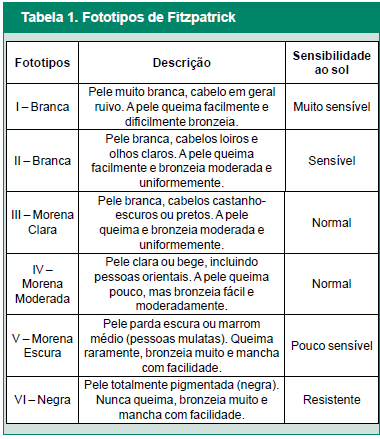
\includegraphics[]{Template_Latex_TCC-UNIFTEC/_lib/imagens/fototipo.png}

\label{fig:x fototipo_fitzpatrick}
\centering{\Fonte{\cite{Régua_de_Pele_Linha_de_Maquiagem_para_a_Mulher_Brasileira}.}}
\end{figure}

Segundo a Sociedade Brasileira de Dermatologia (SBD)\cite{Classificacao-dos-fototipos-de-pele-SBD}, a escala tem aplicabilidade para questões técnico-científicas, como a elaboração do planejamento para tratamento de fototerapia. Contudo, a escala de Fitzpatrick baseia-se, originalmente, a reposta da radiação violeta a pele branca\cite{Classificao_de_fototipos_de_pele} e para o desenvolvimento de \textit{machine learning} ela resultou em viés não intencional que exclui tons mais escuros \cite{Monk_2019}.
 

\subsection{Escala de Monk}
A pesquisa envolta ao desenvolvimento da escala de Monk(MST) tem como um dos objetivos tornar a visão computacional mais inclusiva. A paleta foi criada para substituir o padrão falho das seis cores de Fitzpatrick \cite{Monk_2019}, que, até o momento, é o padrão da indústria de tecnologia para categorizar o tom de pele. Criada pelo Dr. Ellis Monk essa paleta está sendo usada pela empresa Google para promover diversidade e inclusão na tecnologia. Ela fornece um espectro mais amplo de tons de pele que pode ser aproveitado para avaliar conjuntos de dados e modelos de \textit{machine learning} para melhor representação.

A paleta foi desenvolvida com base na pesquisa do Dr. Monk sobre os tons de pele e estudo de colorismo nos Estados Unidos e Brasil, que se concentrava em estudar a variação da exposição geográfica à radiação ultravioleta cria diferentes distribuições de tons de pele entre as populações. A paleta foi avaliada por especialistas em psicologia social e categorização social, bem como comunidades sub-representadas, para saber como eles percebiam a escala. Resultando em uma escala de 10 tons projetada para representar uma gama maior das comunidades.

Recentemente a paleta foi validada como sendo mais inclusiva e com melhor representatividade de tons de pele do que a escala de Fitzpatrick para fins de treinamento de ML. Além disso, também foi avaliado que a escala de Monk é tão representativa quanto uma paleta de beleza de 40 cores \cite{Monk_2019}. As escalas de tom de base de empresas de maquiagem podem incluir mais de 40 tons de pele, isso sem considerar diferenças de tons de produto entre linhas da mesma marca. Porém, quanto maiores as escalas, maior o desafio para casos de uso de ML, devido à dificuldade de aplicar tantos tons consistentemente em uma ampla variedade de conteúdo \cite{Monk_2019}. No caso da classificação do tom de pele, o problema passa a ser mais difícil. Quanto mais tons são agregados com parâmetros mais próximos e semelhantes há impacto na classificação \cite{Automatic_Skin_Tone_Extraction_for_Visagism_Applications}.Sendo assim, os 10 tons possuem granularidade suficiente para refletir uma diversidade de comunidades, sem aumentar a complexidade, permitindo treinamento e avaliação de ML. É importante salientar, que a paleta não planeja identificar uma cor exata de pele, uma vez que a cor da pele humana é extremamente variável e complexa. Ao contrário, o objetivo é assegurar que os pesquisadores possam ver uma medida de tom de pele e encontrar um tom mais próximo.

\section{Tipos de pele brasileira}
O Brasil é um país conhecido por ser miscigenado e por conta disso possui inúmeros tipos de tons de pele. Segundo o \cite{ibge_2022}, na Pesquisa Nacional por Amostra de Domicílios (PNAD) Contínua, 42,8\% dos brasileiros se declararam como brancos, 45,3\% como pardos e 10,6\% como pretos.Não há dados que indiquem qual a tonalidade dos pesquisados, contudo, o Grupo Boticário realizou um estudo que indicou a existência de 168 tons de pele no Brasil, sendo 32 delas correspondentes a 98\% da população \cite{168_tons}, essas informações foram utilizadas para o desenvolvimento de novas cartelas de cores para o grupo atender. 

\section{Visão Computacional}

\section{Processamento digital de imagens}
Da mesma forma que ocorre na detecção de pele, a detecção de cores é sensível a dispositivos de captura e condições de iluminação, como luminosidade, contraste, transparência, brilho e saturação \cite{Human_Skin_Detection_Using_RGB_HSV_and_YCbCr_Color_Models}. Mesmo com pouca alteração de balanço de branco, na cor da pele há diferentes efeitos  em retratos digitais \cite{Skin_Color_Perception_in_Portrait_Image_and_AR_based_Humanoid_Emoji}. Nós humanos somos bons em identificar cores em diferentes iluminações, o que pode ser definido por consistência de cor \cite{Skin_detection_ashort_tutorial}.Contudo, consistência de cor é relativo à percepção, tornando um desafio para a detecção de pele a representação de cores sem a variação e sensibilidade a iluminação. Por isso, o tom da pele é por muitas vezes a combinação de outras características, como textura e recursos de borda. Considerando isso, a detecção de tom de pele para ser otimizada deve considerar a combinação dos fatores mencionados anteriormente em uma faixa de valores ideais, além de considerar as bordas de um rosto, que pode ser obtido a partir da divisão de pixeis de uma imagem em píxeis individuais e classificando-os em regiões de pele e não pele.\cite{Human_Skin_Detection_Using_RGB_HSV_and_YCbCr_Color_Models}.

\subsection{Segmentação de pele}
Usando aprendizado de máquina com base em conjuntos de dados disponíveis, um classificador pode ser treinado para diferenciar um píxel de pele e um sem pele a partir do processo de segmentação, criando  intervalo de valores válidos. Em seguida, um conjunto de áreas da imagem é reconhecido como uma imagem de pele, usando sistemas de cores.

\section{Sistema de Cores}
 Desde a antiguidade, a cor influencia a forma psicológica, fisiológica social e emocional na vida das pessoas \cite{Visagismo}. E a sua percepção é relativa, já que é dependente das relações e interações com outras cores e a tonalidade do fundo \cite{Visagismo}.Por isso, quando se tratando de tratamento de imagens, a escolha do sistema de cores é importante.

Os sistemas de cores ou modelos de cores são modelos matemáticos abstratos que representam as informações de cor por meio de diferentes componentes. A escolha do sistema de cores é crítica para a classificação das cores, cada sistema representa os recursos de cores de maneiras distintas de foram que as cores sejam melhores distinguidas e mais adequadas. Os sistemas de cores mais utilizados no processo de reconhecimento de imagem de pele são o RGB, HSV, Lab e YCbCr\cite{Modelo_matematico_para_reducao} e cada um possuem diferentes aplicações como para processamento de imagem, computação gráfica, exibição de conteúdo e impressões.

No caso da classificação do tom de pele, o problema passa a ser mais difícil. Quanto mais tons são agregados como parâmetro, mais próximos e semelhantes passam a ser as cores, e isso impacta a classificação. Além disso, a rotulagem da cor da pele é muitas vezes considerado subjetiva, mesmo por profissionais treinados \cite{Automatic_Skin_Tone_Extraction_for_Visagism_Applications}
Por isso a escolha do sistema de cor afeta a desempenho de qualquer algoritmo de detecção de tom de pele e qual a sensibilidade às condições de luz \cite{Skin_detection_ashort_tutorial}.Outro desafio se refere a objetos que possuem tons próximos a tons de pele como a madeira, coura, roupas nos tons nude e cabelo. O que pode acarretar detecções com falso positivos quando o ambiente e fundo não são controlados.


\subsection{Modelo RGB}
O sistema de cores RGB (\textit{Red, Green, Blue}) é comumente usado em imagens digitais e se assemelha a codificação de cores do olho humano \cite{Visão_Computacional_Indexação_Automatizada_de_Imagens}. O sistema codifica as cores como uma combinação aditiva de três cores primárias: vermelho (R), verde (G) e azul (B), que representam as frequências baixas, médias e altas, respectivamente, do espectro da luz visível. O espaço de cor formado é um cubo onde nos vértices estão as cores primárias e as secundárias, além da cor preto, para ausência de cores, e o branco, para a presença das 3 cores, conforme a Figura \ref{fig: RGB }. Normalmente, com valores do eixo variando entre 0 a 255 \cite{Cor_Aspectos_relevantes_para_viualização_de_cor}. 

\begin{figure}[h]
\caption{}
\centering

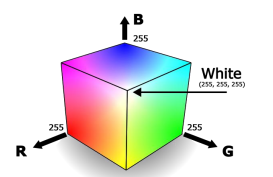
\includegraphics[]{Template_Latex_TCC-UNIFTEC/_lib/imagens/RGB.png}

\label{fig: RGB }
\centering{\Fonte{\cite{}.}}
\end{figure}

Sua principal vantagem é a sua simplicidade. No entanto, o RGB não é perceptivamente uniforme, o que significa que as distâncias no espaço RGB não correspondem linearmente à percepção humana. \cite{Skin_detection_ashort_tutorial}. Além disso, as cores no espectro RGB não separam luminância e crominância, e os componentes R, G e B são altamente correlacionados. A luminância de um determinado píxel RGB é uma combinação linear do R, valores G e B. Portanto, alterar a luminância sobre a pele afeta todos os três componentes. O que conclui que a cor de pele mudará com base na intensidade da iluminação, o que em um tratamento de foto não é o ideal. Apesar dessa limitação, o RGB é extensivamente usado na literatura de detecção de pele devido à sua simplicidade e dependendo do método utilizado pode ter resultados satisfatórios.


 \subsection{Modelo YCbCr}
O modelo YCbCr é uma transformação do espaço RGB \cite{Deteccao_de_pele_humana_em_imagens_veiculadas_na_web}. Neste modelo, as cores são representadas pelo componente Y que supõe-se possuir a informação de luminância, e por dois componentes de crominância, Cb representa a crominância azul e Cr a crominância vermelho, conforme Figura \ref{fig: ycbcr }. Por este motivo podem ter o brilho e a cromaticidade separados. 

\begin{figure}[h]
\caption{}
\centering

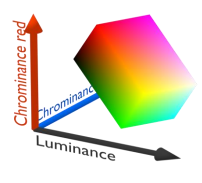
\includegraphics[]{Template_Latex_TCC-UNIFTEC/_lib/imagens/ycbcr.png}

\label{fig: ycbcr }
\centering{\Fonte{\cite{}.}}
\end{figure}

A conversão do espaço RGB para o YCbCr possui vantagens, pois para a visão humana há a sensibilidade maior a luminância. O que possibilita separa e reduzir a quantidade de bits utilizado para a crominância sem perde a qualidade das imagens perante a visão humana. Por conta disso o YCbCr é o modelo bastante utilizado no contexto de imagens digitais e processamento de vídeo.
 
\subsection{Modelo HSV}
O modelo de espaço de cor HSV é um modelo perceptual, ou seja, o espaço descreve a cor mediante atributos relacionados a percepção da coloração\cite{Deteccao_de_pele_humana_em_imagens_veiculadas_na_web}. É baseado em Matiz-Saturação e é também muito utilizado na área de detecção de pele. Esse modelo é separado em três componentes de tonalidade, tonalidade(H), saturação(S) e brilho(V). O componente H descreve a cor dominante como vermelho, verde, azul, de uma área. O componente S mede a coloração de uma área proporcional ao brilho com variações a cor cinza até as cores totalmente saturadas. Já o componente V referir-se a iluminação, conforme ilustrado na Figura\ref{fig: hsv}.

 \begin{figure}[h]
\caption{}
\centering

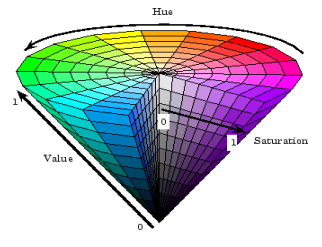
\includegraphics[]{Template_Latex_TCC-UNIFTEC/_lib/imagens/HSV.png}

\label{fig: hsv}
\centering{\Fonte{\cite{}.}}
\end{figure}

 Um dos benefícios deste modelo é que ele permite adicionar a intuitividade e a separação entre tonalidade e saturação, já que o componente V traz a informação de brilho, facilitando a redução de influência de iluminação no tratamento de imagens\cite{Skin_detection_ashort_tutorial}.
 
 \subsection{Modelo CIE-Lab} 
O modelo CIE-lab ou L*a*b é um modelo de cor colométrico definido pela Comitê Internacional de Iluminação (Commission Internationale d’Eclairage - CIE). CIE-Lab é um modelo que separa a luminância(L) das outras duas variáveis de crominância (a,b), conforme Figura \ref{fig: cielab}. Este é um modelo pouco utilizado já que a conversão a partir do RGB é mais cara computacionalmente \cite{Skin_detection_ashort_tutorial} comparado aos outros modelos.

\begin{figure}[h]
\caption{}
\centering

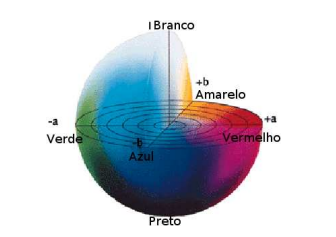
\includegraphics[]{Template_Latex_TCC-UNIFTEC/_lib/imagens/cielab.png}

\label{fig: cielab }
\centering{\Fonte{\cite{}.}}
\end{figure}
 
Segundo o estudo \cite{Automatic_Skin_Tone_Extraction_for_Visagism_Applications}
a precisão da classificação depende de qual sistema de cor é utilizado para a classificação. Para a comparação, a Tabela \ref{table:Tabela_comparativa_sistemas_de_cores} demonstra a relação de sistema de cor e precisão para detecção de tom de pele.

% Please add the following required packages to your document preamble:
% \usepackage{graphicx}
\begin{table}[]
\centering
\caption{Tabela Comparativa Sistemas de Cor}
\label{table:Tabela_comparativa_sistemas_de_cores}\textbf{}
\begin{tabular}{lll}
\hline
  & Sistemas de Cor                   & Precisão \\ \hline
1 & R, G, B                           & 74.65\%  \\
2 & H, S, V                           & 83.30\%  \\
3 & L, a, b                           & 72.46\%  \\
4 & Y, Cr, Cb                         & 83.30\%  \\
5 & L, a, b, H, S, V                  & 85.18\%  \\
6 & L, a, b, Grayscale                & 84.19\%  \\
7 & L, a, b, H, S, R, G, B, Y, Cr, Cb & 86.67\%  \\ \hline
\end{tabular}%
\centering{\Fonte{Autor}}
\end{table}

Frente a diversificada forma de descrever uma tonalidade de pele usando diferentes espaços de cor,neste estudo foram destacados os espaços de cor RGB, YCbCr e HSV, amplamente utilizados em equipamentos de captura (por exemplo câmeras fotográficas e filmadoras digitais). 

O modelo de cor de pele é produzido com base em rostos
individuais.No entanto, a literatura ainda carece de evidências sobre
qual escala é adequada para ser usada como método de detecção
dinâmica da cor da pele.

\subsection{Algoritmo K-means}
Impulsionado não apenas pela indústria cosmética, mas também pela ciência da visão computacional, um esforço significativo foi feito para coletar os verdadeiros valores da cor da pele, principalmente com foco no rosto. Para a identificação do que é pele e não pele em uma imagem se muito utilizado as técnicas de detecção de pele classificadas como técnicas baseadas em píxeis ou técnicas baseadas em regiões. Nessa detecção é classificado como píxel de pele ou não pele individualmente, dependendo de certas condições, como cores e regiões consideradas regiões de pele. Inicialmente a região da pele cresce adicionando mais píxeis com base nas propriedades de seus vizinhos.

\subsection{Algoritmo Haar Cascade}
O algoritmo Haar Cascade, ou algoritmo Viola-Jones, foi proposto por \cite{Viola-Jones} em 2011 e é um método eficaz para detecção de objetos. Possui uma abordagem baseada em \textit{Machine Learning} que funciona com base em cascatear com base no treinamento a partir de muitas imagens positivas e negativas. Em seguida, utilizado para detectar objetos em outras imagens.

O algoritmo Viola-Jones possui três contribuições. A primeira
foi a introdução de uma nova representação de imagem chamada
“Imagem Integral” que permite que as características usadas pelo detector sejam calculadas rápido. A imagem integral pode ser
calculado a partir de uma imagem usando algumas operações por pixel. Uma vez calculado, qualquer um desses recursos \textit{Haar-like features} pode ser calculado em qualquer escala ou local em tempo constante.\cite{Viola-Jones}. As \textit{Haar-like features} são padrões retangulares definidas como a diferença entre a soma das intensidades dos píxeis em duas ou mais regiões retangulares adjacentes em uma imagem. 
A segunda é um algoritmo de \textit{machine learning}, chamado \textit{AdaBoost}, que seleciona um pequeno número de recursos visuais críticos de um conjunto maior e produz classificadores extremamente eficientes. O algoritmo de \textit{boosting} \textit{AdaBoost} possui grande destaque devido ao seu potencial, flexibilidade e simplicidade para ser implementado em diferentes cenários. A terceira contribuição é um método para combinar classificadores cada vez mais complexos em cascata que permite regiões que não são de interesse, como o fundo de imagem, seja descartada rapidamente enquanto o foco se torna processar as regiões promissoras semelhantes aos objetos.

O que resultou em um algoritmo que minimiza ao máximo os custos computacionais mantendo a acurácia da detecção alta\cite{Viola-Jones}. Além disso, o Haar Cascade pode ser encontrado
na biblioteca OpenCV sendo possível utilizar conjuntos disponibilizados em XML para multiplos objetos.

Apesar de ser um algoritmo muito conhecido e utilizado na área de visão computacional, a maior efetividade do algoritmo ainda se dá por conta de imagens frontais de faces. Há ainda a possibilidade de ser reportado faces em imagens onde não existe um rosto realmente, sendo um falso-positivo e também a possibilidade de não reconhecer rosto algum. Como ocorrido no estudo \cite{Classification_Algorithm_for_Skin_Color_CASCo_A_new_tool} na Figura 

\begin{figure}[h]
\caption{Casco }
\centering

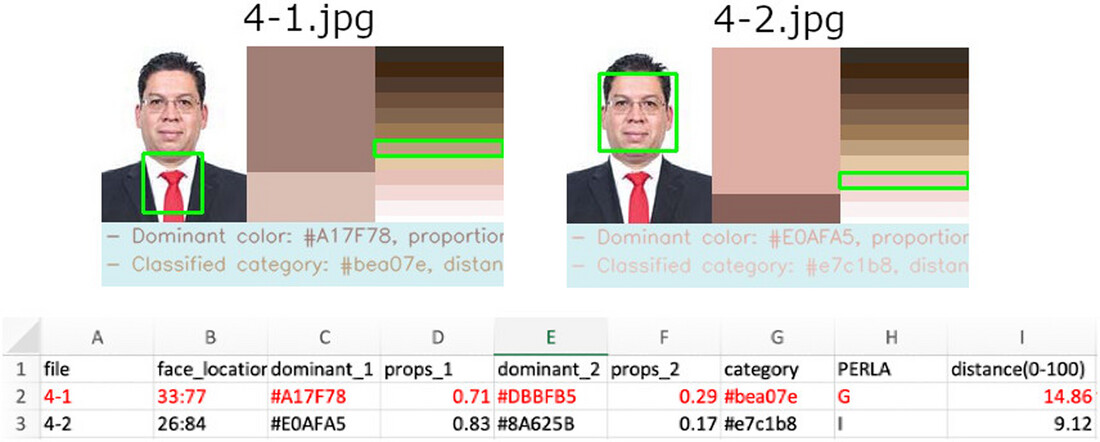
\includegraphics[]{Template_Latex_TCC-UNIFTEC/_lib/imagens/casco.jpg}

\label{fig:x casco-miss-identification}
\centering{\Fonte{\cite{Classification_Algorithm_for_Skin_Color_CASCo_A_new_tool}.}}
\end{figure}
\subsection{Segmentação de Pele}
\section{Visão Computacional}


O processo de identificação de cor de pele é uma das etapas para a identificação de pele. Apesar disso. a detecção de coloração de pele continua sendo um desafio para o processamento de imagem \cite{Human_Skin_Color_Detection_Technique_Using_Different_Color_Models}. Já que a coloração é criada baseada na combinação de sangue (cor vermelha) e melanina (cor amarela e marrom). \cite{Human_Skin_Color_Detection_Technique_Using_Different_Color_Models}.Recentemente, com os novos desenvolvimentos em visão computacional vários trabalhos tentaram classificar a cor da pele a partir de imagens. Apesar de, utilizando imagens a detecção da cor da pele fica suscetível a influência de vários fatores, como características da câmera, etnia, sombras, iluminação, cores de fundo de movimento\cite{Human_Skin_Detection_Using_Different_Color_Spaces}.
 
Quanto mais tons de cor da pele são utilizados para classificação, mais os tons estão próximos uns dos outros e mudanças de iluminação tornam a cor ainda mais difícil de diferir.Embora, no campo da dermatologia e antropometria, acor da pele é classificada em um nível alto de granularidade , sendo de 6 e 36 tons de pele, respectivamente \cite{Automatic_Skin_Tone_Extraction_for_Visagism_Applications}. Esquemas de classificação mais complexos são altamente subjetivo e apresenta problemas mesmo para
praticantes humanos. Um modelo com seis cores seria provavelmente seria ideal, pois os seis tons combinariam
o que podemos distinguir visualmente entre diferentes
regiões e raças humanas como cores de pele predominantes.
No entanto, estudos práticos (Boaventura et al., 2006)
mostram que a classificação natural e não influenciada de
as cores da pele executadas por humanos conteriam
apenas três classes: branco/claro, pardo e preto.
Porém, mesmo com três turmas, a classificação é
subjetivo




\label{cap:fundamentacao-teorica}